\graphicspath{{chapters/03/media/}}
\chapter{Processamento dei dati}
\label{cha:processamento}
Dopo aver definito in \S\ref{cha:intro} l'obiettivo di questo progetto si deve definire una pipeline che, da dati di sequenziamento di RNA e di \emph{WES}\footnote{SEMPRE DEFINITO NEL CAPITOLO 1} sia in grado di fornire le istanze di espressione allelo-specifica.
Questa pipeline viene definita basandosi su quella presentata in \cite{ase_pipeline} e si compone pertanto di tre fasi principali:
\begin{enumerate}
	\item Pre-processamento e allineamento dei dati di RNA-seq, con eventuale deduplicazione e ricalibrazione.
	\item Analisi di dati \emph{WES} in modo da ottenere una lista di possibili SNP esonici da considerare.
	\item Ottenimento dei dati di sbilanciamento allelico.
\end{enumerate}
La figura \ref{fig:proj_pipeline} \`e una visualizzazione della pipeline e dei tool utilizzati.\\
Essendo infine che questo lavoro prevede il processamento di un gran numero di file, unito al fatto che i tool utilizzzati sono stati implementati con una integrazione con le pipe di unix e con la possibilit\`a di essere eseguiti in multi-threading \`e stato di fondamentale importanza l'utility parallel \cite{parallel}.
In particolare nel caso di STAR\footnote{\S\ref{subsec:star}} \`e stato notato una diminuzione lineare delle performance per thread del tool.
L'abbassamento delle performance \`e stato risolto grazie a parallel, lanciando pi\`u istanze parallele del tool, ognuna di esse con pochi thread.
Si nota pertanto che parallel permette non solo un'elegante implementazione della pipeline, ma fornisce un livello di controllo tale da sfruttare completamente la potenza computazionale disponibile, riducendo in questo modo il tempo globale di esecuzione.


  \begin{figure}[H]
    \label{fig:proj_pipeline}
    \centering
    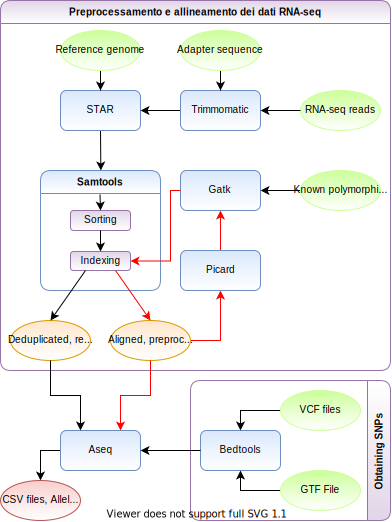
\includegraphics[scale=0.2]{pipeline.png}
    \caption{Pipeline per l'ottenimento dei dati di allelic imbalance}
  \end{figure}

  \section{Pre-processamento e allineamento dei dati RNA-seq}
  \label{sec:pre_all_rna_seq}
  Il primo passo della pipeline appenda definita \`e il pre-processamento e l'allineamento dei dati RNA-seq.
  L'input della pipeline sono dei file \emph{FASTQ}, ovvero file di testo che contengono i dati di sequenziamento raccolti in laboratorio tipicamente compressi.
  Questi file vengono modificati dai tool Trimmomatic, Star e Samtools in modo da produrre un output gi\`a utilizzabile per ottenere i dati di sbilanciamento allelico.
  Opzionalmente l'output pu\`o subire ulteriori modifiche prima di passare alla prossima fase: in particolare pu\`o essere deduplicato e ricalibrato.

  	\subsection{Trimmomatic}
	Trimmomatic \cite{trimmomatic} \`e il primo tool ad essere utilizzato.
	Il suo obiettivo \`e quello di eliminare dalle reads la sequenza adattatrice, o suoi frammenti, utilizzata per rendere possibile il sequenziamento.
	Essendo le RNA-seq fornite a single-ends\footnote{Spiega cosa sono} viene utilizzata la simple mode del tool.
	Questa scansiona ogni read\footnote{Non so se metterla in italiano} dalla terminazione $5'$ alla $3'$ per determinare la presenza della sequenza adattatrice.
	Utilizza il mdetodo ``seed and extend'' per trovare corrispondenze iniziali, anche non perfette, tra la read e la sequenza adattatrice.
	Successivamente svolge un allineamento locale e se questo ha uno score maggiore di una soglia viene rimosso insieme alla porzione successiva ad esso.
	Questa modalit\`a permette di identificare ogni sequenza adattatrice in ogni luogo della read a patto che l'allineamento sia abbastanza lungo e la read abbastanza accurata.
	Si nota per\`o come nelle regioni dove solo una corta corrispondenza parziale \`e possibile come alle estremit\`a della read e pertanto i contaminanti non possono essere identificati attendibilmente.
	Oltre alla rimozione delle sequenze adattatrici Trimmomatic tronca un'estremit\`a secondo un algoritmo di filtraggio secondo qualit\`a.
	Tra i metodi forniti dallo strumento \`e stato utilizzato quello del ``sliding window quality filtering'':
	scansiona la read dal $5'$ e rimuove la terminazione $3'$ quando la qualit\`a media di un gruppo di basi scende sotto una soglia specificata.
	Il risultato di questo passaggio sar\`a un altro fastq file con le sequenze adattatrici rimosse.

	\subsection{Star}
	\label{subsec:star}
	Star (spliced transcript alignment to a reference) \cite{star} \`e il secondo tool della pipeline.
	Prende come input il file fastq generato da Trimmomatic e un genoma di reference\footnote{Anche qui lo lascio in italiano?} e allineando il primo al secondo.
	Questo tool \`e stato creato con l'obiettivo di allineare RNA-seq di media-grande lunghezza, a differenza dei suoi competitori che, essendo creati a partire da allineatori per dati di DNA, hanno un maggiore tasso di errore.
	Questo avviene a causa degli eventi di splicing che avvengono nella creazione delle molecole di mRNA.
	Star pertanto si prefigge di permettere un allineamento accurato di reads che contengono mal-accoppiamenti, inserzioni o delezioni causati da variazioni genomiche o errori di sequenziamento mappando contemporaneamente sequenze derivate da regioni genomiche non contigue unite da eventi di splicing.
	Per farlo utilizza un algoritmo in due fasi.
	La prima fase o \emph{seed search} consiste della ricerca sequenziale di \emph{Maximal Mappable Prefix MMP}.
	Data una sequenza $R$, una regione $i$ e un genoma di reference $G$, $MMP(R, i, G)$ \`e la pi\`u lunga sottostringa $(R_i, R_{i+1}, \dots, R_{i+MMK-1})$ che corrisponde esattamente a una o pi\`u sottostringhe di $G$.
	$MML$ \`e la massima lunghezza mappabile.
	Questo permette un'identificazione di giunzioni di splicing senza nessuna conoscenza a priori.
	L'implementazione attraverso \emph{Uncompressed suffix arrays} causa alla complessit\`a dell'algoritmo di scalare logaritmicamente con la lunghezza del genoma di reference.
	Gli array sono non compressi per permettere tempi di ricerca pi\`u veloci, ma causano un aumento del consumo di memoria.
	La seconda fase o \emph{clustering, stitching and scoring} consiste nel costruire allineamenti dell'intera sequenza di reads unendo tutti i seed allineati al genoma nella prima fase.
	In primo luogo i seed sono raggruppati insieme secondo la vicinanza a un seed ancora selezionato limitando il numero di loci genomici a cui questo si allinea.
	Successivamente tutti i seed mappati nella \emph{genomic window} sono uniti insieme assumendo un modello lineare locale di trascrizione.
	Questo processo di unione viene inoltre guidato da un sistema di punteggi che penalizza mal-accoppiamenti, inserzioni, delezioni e \emph{splice junction gap}.
	Star ha come output un sam file, un file di testo delimitato da tabulazioni contenente una riga per allineamento con tutte le informazioni necessarie per la sua identificazione.

	\subsection{Samtools}
  I samtools\footnote{Necessario citare i siti della documentazione} sono un insieme di programmi necessari per interagire con i dati di sequenziamento.
  Nella pipeline sono utilizzati per compiere delle operazioni sui sam file generati da Star\footnote{Mettere riferimento a Star} in modo da prepararli prima che possano essere utilizzati successivamente da ASEQ\footnote{Riferimento ad ASEQ}.
  In particolare svolgono le operazioni di ordinamento, indicizzazione e compressione dei file di input.
  Questo avviene attraverso due programmi: samtools sort e samtools index.
  Il primo ordina gli allineamenti secondo le coordinate di inizio e comprime implicitamente l'input in formato bam.
  Il secondo invece crea, a partire dall'output del programma sort un indice in formato bai di tale file, permettendo efficienti operazioni di accesso casuale al bam file.
  L'output finale \`e un bam file ordinato e indicizzato che pu\`o essere utilizzato come input di ASEQ\footnote{riferimento ad aseq} per generare i dati di sbilanciamento allelico.

	\subsection{Deduplicazione e ricalibrazione}
  La deduplicazione e la ricalibrazione sono due processi ulteriori di pre-processamento dei dati che tentano di risolvere errori presenti nei bam file che sono stati allineati attraverso star\footnote{Riferimento a star}.
  Questi due passaggi vengono svolti attraverso una serie di tools eseguiti sequenzialmente come si nota nella figura \ref{fig:pipeline_deduprecal}.
  \begin{figure}[H]
    \label{fig:pipeline_deduprecal}
    \centering
    \includegraphics[scale=0.17]{deduprecal.png}
    \caption{Pipeline di deduplicazione e ricalibrazione}
  \end{figure}

    \subsubsection{Deduplicazione}
    Si definiscono come read duplicate in un BAM file delle read che si generano da un singolo frammento di RNA.
    Possono originarsi durante la preparazione del campione, per esempio durante la costruzione della libreria attravero PCR o risultare da un singolo cluster di amplificazione, identificato incorrettamente come cluster multipli dal sensore ottico dello strumento di sequenziamento.


  \section{Analisi dei dati WES}

  	\subsection{Bedtools}

  \section{Dati disponibili}
  \label{sec:dati}

    \subsection{Sequenze biologiche}
    \label{subsec:fastq}

    Descrizione dei fastq.

    \subsection{Genoma di riferimento}
    \label{subsec:star-gen}
    Descrizione del genoma di riferimento.

    \subsection{Variant call}
    \label{subsec:vcf}
    Descrizione dei vcf.

    \subsection{Struttura dei geni}
    \label{subsec:gtf}
    Descrizione del gtf.

  \section{Troncatura e allinamento}
  \label{sec:trimm_star}
  Descrizione del processo e perch\`e viene fatto.

    \subsection{Troncatura}
    \label{subsec:trimm}
    Trimmomatic, cosa fa come \`e stato usato.

    \subsection{Allineamento}
    STAR, cosa fa come \`e stato usato.

    \subsection{Ordinamento}
    \label{subsec:sorting}
    SAMTOOLS SORT cosa fa come \`e stato usato.

    \subsection{Indicizzazione}
    \label{subsec:indexing}
    SAMTOOLS index cosa fa come \`e stato usato.

  \section{Deduplicazione, riallinamento e recalibrazione}
  \label{sec:recalibration}
  Descrizione del processo e perch\`e viene fatto

    \subsection{Deduplicazione}
    \label{subsec:dedup}
    Come sopra.

    \subsection{Riallineamento e recalibrazione}
    \label{subsec:recalibration}
    Come sopra.

  \section{Ottenere le varianti alleliche}
  Intersezione tra VCF e GTF.

  \section{Ottenere i dati delle frazioni alleliche}
  \label{sec:aseq}
  ASEQ cosa fa come viene usato.


    \subsection{Filtrare le frazioni alleliche}
    \label{subsec:filter}
    Condizioni di filtraggio per i risultati di ASEQ.

  \section{Ottenere gli SNP nel 3'-UTR}
  \label{sec:threeprime}
  Filtraggio del gtf e intersezione con i VCF
